\documentclass{standalone}
\usepackage{tikz}
\usetikzlibrary{patterns, positioning}


\begin{document}
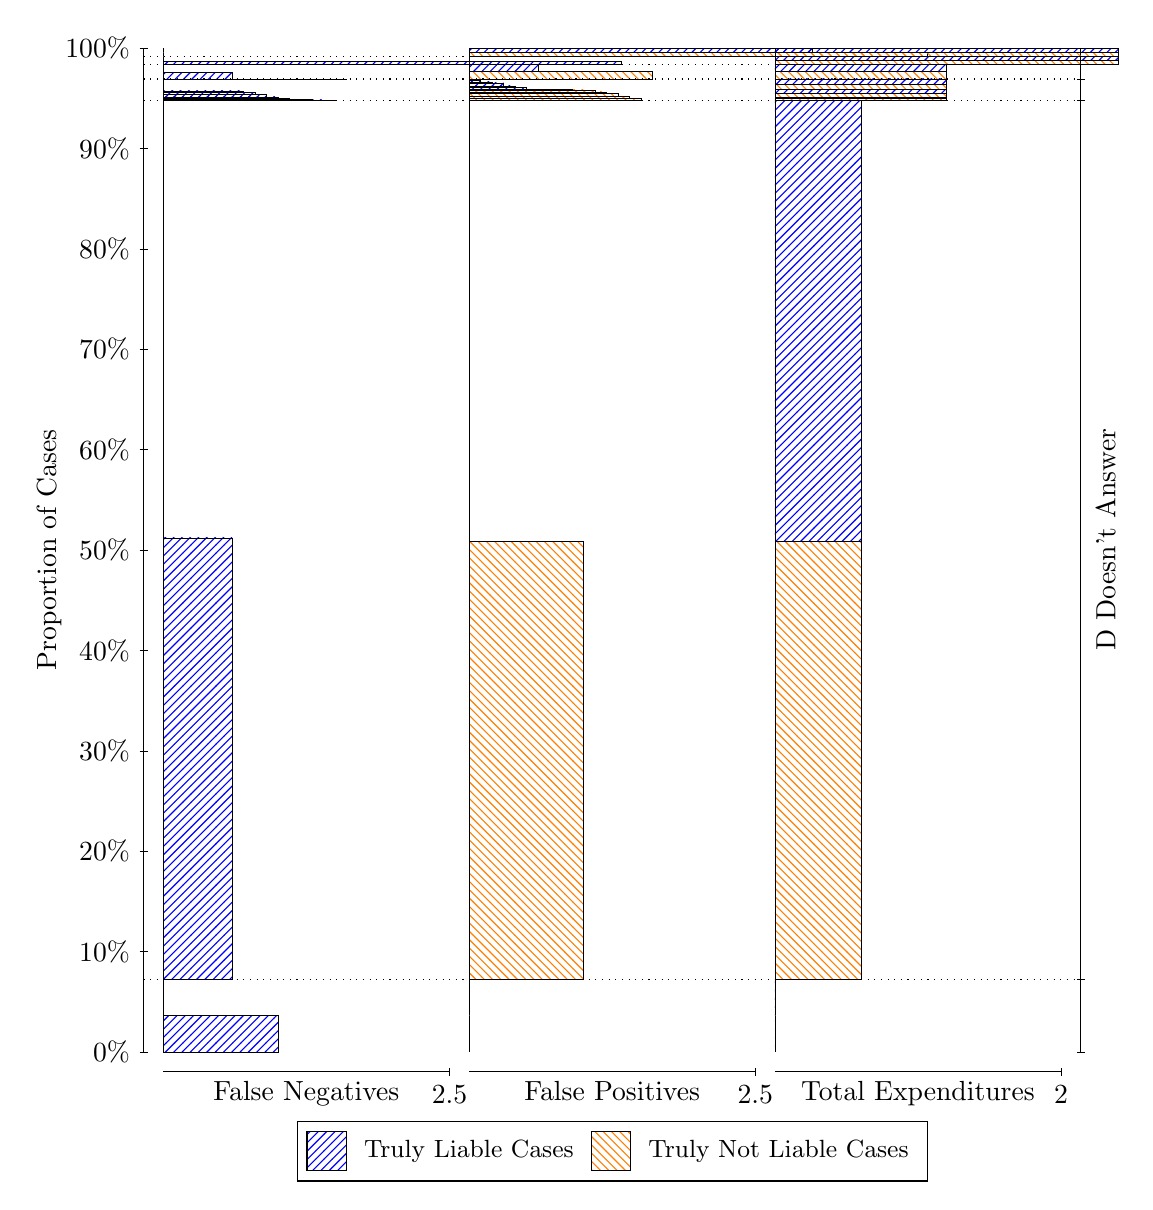
\begin{tikzpicture}
\draw[black, very thin] (1.5,1.75) -- (1.5,14.5);
\node[rotate=90, text=black, anchor=center] at (0.3, 8.125) {Proportion of Cases};
\draw[black, very thin] (1.45,1.75) -- (1.55,1.75);
\node[text=black, anchor=east] at (1.45, 1.75) {0\%};
\draw[black, very thin] (1.45,3.025) -- (1.55,3.025);
\node[text=black, anchor=east] at (1.45, 3.025) {10\%};
\draw[black, very thin] (1.45,4.3) -- (1.55,4.3);
\node[text=black, anchor=east] at (1.45, 4.3) {20\%};
\draw[black, very thin] (1.45,5.575) -- (1.55,5.575);
\node[text=black, anchor=east] at (1.45, 5.575) {30\%};
\draw[black, very thin] (1.45,6.85) -- (1.55,6.85);
\node[text=black, anchor=east] at (1.45, 6.85) {40\%};
\draw[black, very thin] (1.45,8.125) -- (1.55,8.125);
\node[text=black, anchor=east] at (1.45, 8.125) {50\%};
\draw[black, very thin] (1.45,9.4) -- (1.55,9.4);
\node[text=black, anchor=east] at (1.45, 9.4) {60\%};
\draw[black, very thin] (1.45,10.675) -- (1.55,10.675);
\node[text=black, anchor=east] at (1.45, 10.675) {70\%};
\draw[black, very thin] (1.45,11.95) -- (1.55,11.95);
\node[text=black, anchor=east] at (1.45, 11.95) {80\%};
\draw[black, very thin] (1.45,13.225) -- (1.55,13.225);
\node[text=black, anchor=east] at (1.45, 13.225) {90\%};
\draw[black, very thin] (1.45,14.5) -- (1.55,14.5);
\node[text=black, anchor=east] at (1.45, 14.5) {100\%};

\draw[black, very thin] (13.4,1.75) -- (13.4,14.5);
\draw[black, very thin] (13.35,1.75) -- (13.45,1.75);
\node[anchor=west] at (13.35, 1.75) {};
\draw[black, very thin] (13.35,2.6745) -- (13.45,2.6745);
\node[anchor=west] at (13.35, 2.6745) {};
\draw[black, very thin] (13.35,13.836) -- (13.45,13.836);
\node[anchor=west] at (13.35, 13.836) {};
\draw[black, very thin] (13.35,14.099) -- (13.45,14.099);
\node[anchor=west] at (13.35, 14.099) {};
\draw[black, very thin] (13.35,14.109) -- (13.45,14.109);
\node[anchor=west] at (13.35, 14.109) {};
\draw[black, very thin] (13.35,14.288) -- (13.45,14.288);
\node[anchor=west] at (13.35, 14.288) {};
\draw[black, very thin] (13.35,14.395) -- (13.45,14.395);
\node[anchor=west] at (13.35, 14.395) {};
\draw[black, very thin] (13.35,14.5) -- (13.45,14.5);
\node[anchor=west] at (13.35, 14.5) {};

\draw[black, very thin, pattern color=blue, pattern=north east lines] (1.75,1.75) rectangle (3.2033,2.2123);
\draw[black, very thin, pattern color=orange, pattern=north west lines] (1.75,2.2123) rectangle (1.75,2.6745);
\draw[black, very thin, pattern color=blue, pattern=north east lines] (1.75,2.6745) rectangle (2.622,8.2775);
\draw[black, very thin, pattern color=orange, pattern=north west lines] (1.75,8.2775) rectangle (1.75,13.836);
\draw[black, very thin, pattern color=blue, pattern=north east lines] (1.75,13.836) rectangle (3.93,13.838);
\draw[black, very thin, pattern color=blue, pattern=north east lines] (1.75,13.838) rectangle (3.7847,13.84);
\draw[black, very thin, pattern color=blue, pattern=north east lines] (1.75,13.84) rectangle (3.6393,13.844);
\draw[black, very thin, pattern color=blue, pattern=north east lines] (1.75,13.844) rectangle (3.494,13.848);
\draw[black, very thin, pattern color=blue, pattern=north east lines] (1.75,13.848) rectangle (3.3487,13.864);
\draw[black, very thin, pattern color=blue, pattern=north east lines] (1.75,13.864) rectangle (3.2033,13.879);
\draw[black, very thin, pattern color=blue, pattern=north east lines] (1.75,13.879) rectangle (3.058,13.915);
\draw[black, very thin, pattern color=blue, pattern=north east lines] (1.75,13.915) rectangle (2.9127,13.938);
\draw[black, very thin, pattern color=blue, pattern=north east lines] (1.75,13.938) rectangle (2.7673,13.957);
\draw[black, very thin, pattern color=orange, pattern=north west lines] (1.75,13.957) rectangle (1.75,14.099);
\draw[black, very thin, pattern color=blue, pattern=north east lines] (1.75,14.099) rectangle (4.0753,14.104);
\draw[black, very thin, pattern color=orange, pattern=north west lines] (1.75,14.104) rectangle (1.75,14.109);
\draw[black, very thin, pattern color=blue, pattern=north east lines] (1.75,14.109) rectangle (2.622,14.193);
\draw[black, very thin, pattern color=orange, pattern=north west lines] (1.75,14.193) rectangle (1.75,14.288);
\draw[black, very thin, pattern color=blue, pattern=north east lines] (1.75,14.288) rectangle (7.5633,14.334);
\draw[black, very thin, pattern color=orange, pattern=north west lines] (1.75,14.334) rectangle (1.75,14.395);
\draw[black, very thin, pattern color=orange, pattern=north west lines] (1.75,14.395) rectangle (1.75,14.446);
\draw[black, very thin, pattern color=blue, pattern=north east lines] (1.75,14.446) rectangle (1.75,14.5);
\draw[black, very thin, pattern color=orange, pattern=north west lines] (5.6333,1.75) rectangle (5.6333,2.2123);
\draw[black, very thin, pattern color=blue, pattern=north east lines] (5.6333,2.2123) rectangle (5.6333,2.6745);
\draw[black, very thin, pattern color=orange, pattern=north west lines] (5.6333,2.6745) rectangle (7.0867,8.233);
\draw[black, very thin, pattern color=blue, pattern=north east lines] (5.6333,8.233) rectangle (5.6333,13.836);
\draw[black, very thin, pattern color=orange, pattern=north west lines] (5.6333,13.836) rectangle (7.8133,13.856);
\draw[black, very thin, pattern color=orange, pattern=north west lines] (5.6333,13.856) rectangle (7.668,13.884);
\draw[black, very thin, pattern color=orange, pattern=north west lines] (5.6333,13.884) rectangle (7.5227,13.927);
\draw[black, very thin, pattern color=orange, pattern=north west lines] (5.6333,13.927) rectangle (7.3773,13.944);
\draw[black, very thin, pattern color=orange, pattern=north west lines] (5.6333,13.944) rectangle (7.232,13.964);
\draw[black, very thin, pattern color=orange, pattern=north west lines] (5.6333,13.964) rectangle (7.0867,13.968);
\draw[black, very thin, pattern color=orange, pattern=north west lines] (5.6333,13.968) rectangle (6.9413,13.973);
\draw[black, very thin, pattern color=orange, pattern=north west lines] (5.6333,13.973) rectangle (6.796,13.975);
\draw[black, very thin, pattern color=orange, pattern=north west lines] (5.6333,13.975) rectangle (6.6507,13.977);
\draw[black, very thin, pattern color=blue, pattern=north east lines] (5.6333,13.977) rectangle (6.36,13.997);
\draw[black, very thin, pattern color=blue, pattern=north east lines] (5.6333,13.997) rectangle (6.2147,14.02);
\draw[black, very thin, pattern color=blue, pattern=north east lines] (5.6333,14.02) rectangle (6.0693,14.056);
\draw[black, very thin, pattern color=blue, pattern=north east lines] (5.6333,14.056) rectangle (5.924,14.071);
\draw[black, very thin, pattern color=blue, pattern=north east lines] (5.6333,14.071) rectangle (5.7787,14.087);
\draw[black, very thin, pattern color=blue, pattern=north east lines] (5.6333,14.087) rectangle (5.6333,14.099);
\draw[black, very thin, pattern color=orange, pattern=north west lines] (5.6333,14.099) rectangle (6.5053,14.104);
\draw[black, very thin, pattern color=blue, pattern=north east lines] (5.6333,14.104) rectangle (5.6333,14.109);
\draw[black, very thin, pattern color=orange, pattern=north west lines] (5.6333,14.109) rectangle (7.9587,14.204);
\draw[black, very thin, pattern color=blue, pattern=north east lines] (5.6333,14.204) rectangle (6.5053,14.288);
\draw[black, very thin, pattern color=orange, pattern=north west lines] (5.6333,14.288) rectangle (5.6333,14.349);
\draw[black, very thin, pattern color=blue, pattern=north east lines] (5.6333,14.349) rectangle (5.6333,14.395);
\draw[black, very thin, pattern color=orange, pattern=north west lines] (5.6333,14.395) rectangle (11.447,14.446);
\draw[black, very thin, pattern color=blue, pattern=north east lines] (5.6333,14.446) rectangle (9.9933,14.5);
\draw[black, very thin, pattern color=orange, pattern=north west lines] (9.5167,1.75) rectangle (9.5167,2.2123);
\draw[black, very thin, pattern color=blue, pattern=north east lines] (9.5167,2.2123) rectangle (9.5167,2.6745);
\draw[black, very thin, pattern color=orange, pattern=north west lines] (9.5167,2.6745) rectangle (10.607,8.233);
\draw[black, very thin, pattern color=blue, pattern=north east lines] (9.5167,8.233) rectangle (10.607,13.836);
\draw[black, very thin, pattern color=orange, pattern=north west lines] (9.5167,13.836) rectangle (11.697,13.856);
\draw[black, very thin, pattern color=blue, pattern=north east lines] (9.5167,13.856) rectangle (11.697,13.873);
\draw[black, very thin, pattern color=orange, pattern=north west lines] (9.5167,13.873) rectangle (11.697,13.924);
\draw[black, very thin, pattern color=blue, pattern=north east lines] (9.5167,13.924) rectangle (11.697,13.97);
\draw[black, very thin, pattern color=orange, pattern=north west lines] (9.5167,13.97) rectangle (11.697,14.04);
\draw[black, very thin, pattern color=blue, pattern=north east lines] (9.5167,14.04) rectangle (11.697,14.099);
\draw[black, very thin, pattern color=orange, pattern=north west lines] (9.5167,14.099) rectangle (11.697,14.104);
\draw[black, very thin, pattern color=blue, pattern=north east lines] (9.5167,14.104) rectangle (11.697,14.109);
\draw[black, very thin, pattern color=orange, pattern=north west lines] (9.5167,14.109) rectangle (11.697,14.204);
\draw[black, very thin, pattern color=blue, pattern=north east lines] (9.5167,14.204) rectangle (11.697,14.288);
\draw[black, very thin, pattern color=orange, pattern=north west lines] (9.5167,14.288) rectangle (13.877,14.349);
\draw[black, very thin, pattern color=blue, pattern=north east lines] (9.5167,14.349) rectangle (13.877,14.395);
\draw[black, very thin, pattern color=orange, pattern=north west lines] (9.5167,14.395) rectangle (13.877,14.446);
\draw[black, very thin, pattern color=blue, pattern=north east lines] (9.5167,14.446) rectangle (13.877,14.5);
\draw[black, dotted] (1.5,2.6745) -- (13.4,2.6745);
\draw[black, dotted] (1.5,13.836) -- (13.4,13.836);
\draw[black, dotted] (1.5,14.099) -- (13.4,14.099);
\draw[black, dotted] (1.5,14.109) -- (13.4,14.109);
\draw[black, dotted] (1.5,14.288) -- (13.4,14.288);
\draw[black, dotted] (1.5,14.395) -- (13.4,14.395);
\draw[black, very thin] (1.75,1.5) -- (5.3833,1.5);
\node[text=black, anchor=north] at (3.5667, 1.5) {False Negatives};
\draw[black, very thin] (5.3833,1.45) -- (5.3833,1.55);
\node[text=black, anchor=north] at (5.3833, 1.45) {2.5};

\draw[black, very thin] (5.6333,1.5) -- (9.2667,1.5);
\node[text=black, anchor=north] at (7.45, 1.5) {False Positives};
\draw[black, very thin] (9.2667,1.45) -- (9.2667,1.55);
\node[text=black, anchor=north] at (9.2667, 1.45) {2.5};

\draw[black, very thin] (9.5167,1.5) -- (13.15,1.5);
\node[text=black, anchor=north] at (11.333, 1.5) {Total Expenditures};
\draw[black, very thin] (13.15,1.45) -- (13.15,1.55);
\node[text=black, anchor=north] at (13.15, 1.45) {2};


\node[text=black, centered, rotate=90] at (13.72, 8.2553) {D Doesn't Answer};






\draw (7.449999999999999,1.5) node[draw=none] (baseCoordinate) {};
\begin{scope}[align=center]
        \matrix[scale=0.5, draw=black, below=0.5cm of baseCoordinate, nodes={draw}, column sep=0.1cm]{
            \node[rectangle, draw, minimum width=0.5cm, minimum height=0.5cm, pattern color=blue, pattern=north east lines] {}; &
            \node[draw=none, font=\small, text=black] (B) {Truly Liable Cases}; &
            \node[rectangle, draw, minimum width=0.5cm, minimum height=0.5cm, pattern color=orange, pattern=north west lines] {}; &
            \node[draw=none, font=\small, text=black] (B) {Truly Not Liable Cases}; \\
            };
\end{scope}

\end{tikzpicture}
\end{document}